\documentclass[tikz,border=10pt]{standalone}
\usepackage{amsmath}
\usetikzlibrary{arrows.meta,positioning,fit,shapes,calc}

\tikzset{
  var/.style={minimum size=8mm,inner sep=0pt,font=\small},
  arrow/.style={-{Latex[length=2pt,width=2pt]},thick}
}

\begin{document}
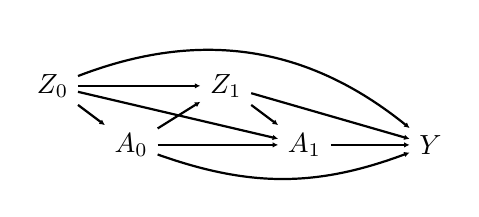
\begin{tikzpicture}

  \node[] (L1) at (1.0,  0.0)  {$Z_0$};
  \node[] (L2) at (3.2,  0.0)  {$Z_1$};
  \node[] (A1) at (2.0, -.75)  {$A_0$};
  \node[] (A2) at (4.2, -.75)  {$A_1$};
  \node[] (Yb) at (5.8, -.75)  {$Y$};

  \draw[arrow] (L1) -- (A1);
  \draw[arrow] (L1) -- (L2);
  \draw[arrow] (L1) -- (A2);
  \draw[arrow] (L1) to[bend right=-30] (Yb);
  \draw[arrow] (A1) -- (L2);
  \draw[arrow] (A1) -- (A2);
  \draw[arrow] (A1) to[bend right=20] (Yb);
  \draw[arrow] (L2) -- (A2);
  \draw[arrow] (L2) -- (Yb);
  \draw[arrow] (A2) -- (Yb);

\end{tikzpicture}
\end{document}
